\documentclass{article}
\usepackage{mathrsfs}
\usepackage{amsmath}
\usepackage{amssymb}
\usepackage{braket}
\usepackage{xcolor}
\usepackage{enumitem}
\usepackage{float}
\usepackage[noend]{algorithm2e}
\usepackage[normalem]{ulem} % for strikeout line
\usepackage{graphicx}
\graphicspath{ {./images/} }
% \usepackage{epstopdf}

%-------------------------------------------------------%
\newcounter{pcounter}                                   %
\newenvironment{problem}                                %
{                                                       %
    \color{gray}                                        %
    \stepcounter{pcounter}                              %
    \textbf{\arabic{pcounter}.}                         %
}{}                                                     %
\newenvironment{solution}                               %
{\textbf{Solution:} }{$\blacksquare$}                   %
%-------------------------------------------------------%
\newcommand{\tab}{\ \ \ \ }                             %
\newcommand{\leadto}{\Rightarrow}                       %
\newcommand{\domR}{\mathcal{R}}                         %
\newcommand{\domS}{\mathbb{S}}                          %
\newcommand{\Gaussian}{\mathcal{N}}                     %
\newcommand{\IdenMat}{\textit{I}}                       %
\newcommand{\abss}[1]{\| #1 \|}                         %
\newcommand{\tr}[1]{\textbf{tr}(#1)}                    %
\newcommand{\vecOne}{\textbf{1}}                        %
%-------------------------------------------------------%

\begin{document}
    %------------------- The Title -------------------%
    \parindent 0in
    \parskip 1em
    \title{COMP9501 Assignment 2 Solution Sheet}
    \author{HONG Yuncong, 3030058647}
    \maketitle

    \begin{section}{Problem 1}
        \setcounter{pcounter}{0}
        %=================== Problem 1.1 ===================%
        \begin{problem}
            [Conditional Independence and Bayes Ball Algorithm]\\
            We have discussed in class how to model conditional independence using graphical models, and how to check the conditional independence between two variable nodes in a grphical model using the Bayes ball algorithm. Answer the questions below, and use either \textit{Bayes Ball algorithm} or \textit{conditional probability} to explain. If you use Bayes ball, please describe the path that the 'ball' takes and give an intuition using the \textit{canonical three-node graph} structures about why (or not) the reachability argument holds, and thus the conditional independence is not satisfied or vice versa.\\
            Considering the model in Figure 1, where the random variables conditioning on are not shaded because they change based on the problem.
            \begin{enumerate}[label=(\alph*)]
                \item Is $X_1 \perp X_2 | X_3$ ?
                \item Is $X_1 \perp X_2 | X_4$ ?
                \item Is $X_1 \perp X_2$ ?
            \end{enumerate}
            \begin{figure}[H]
                \label{fig:m1}
                \centering
                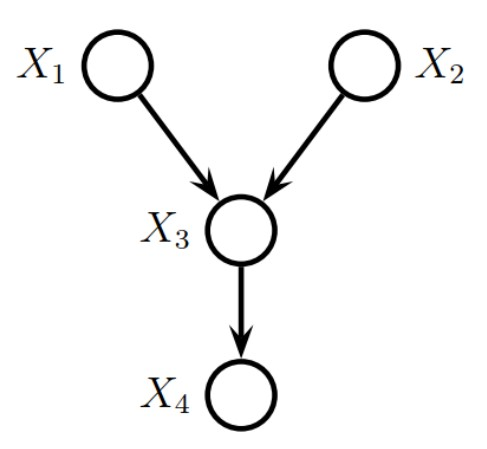
\includegraphics[width=0.37\textwidth]{a2_p11_1}
                \caption{The first graphical model}
            \end{figure}

            Considering the model in Figure 2, where the random variables that are conditioning on are not shaded because they change based on the problem.
            \begin{figure}[H]
                \label{fig:m2}
                \centering
                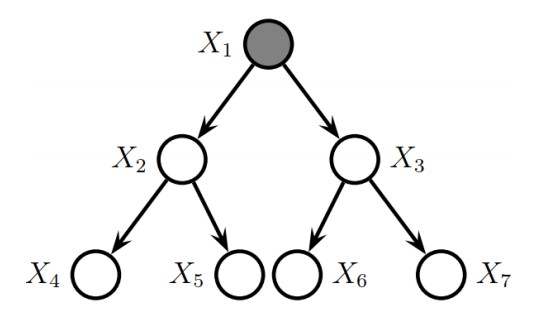
\includegraphics[width=0.5\textwidth]{a2_p11_2}
                \caption{The second graphical model}
            \end{figure}
            \begin{enumerate}[label=(\alph*), resume]
                \item Is $X_4 \perp X_7 | X_1$ ?
                \item Is $X_4 \perp X_5 | X_1$ ?
            \end{enumerate}
        \end{problem}

        \begin{solution}
            \begin{enumerate}[label=(\alph*)]
                \item No, $X_1 \not\perp X_2 | X_3$; As $X_1, X_2, X_3$ form one Fork graph, the ball could move along $X_1 \to X_3 \to X_2$, or $X_2 \to X_3 \to X_1$, with the observation state $X_3$;
                
                \item No, $X_1 \not\perp X_2 | X_4$; As $X_1, X_3, X_4, X_2$ form one V-strusture graph, the ball could move along $X_1 \to X_3 \to X_4 \to X_3 \to X_Z$, with the observation state $X_4$;
                
                \item Yes, $X_1 \perp X_2$; because $Pr(X_1) Pr(X_2) = \frac{Pr(X_1, X_2, X_3)}{Pr(X_3|X_1, X_2)} = \frac{Pr(X_1) Pr(X_2) Pr(X_3|X_1,X_2) }{Pr(X_3|X_1, X_2)} = Pr(X, Y)$;
                
                \item No, $X_4 \not\perp X_7 | X_1$; condition is not complete because:
                \begin{align*}
                    Pr(X_4, X_7 | X_1, X_2, X_3) &=
                    \frac{Pr(X_1, X_2, X_3, X_4, X_5)}{Pr(X_1) Pr(X_2|X_1) Pr(X_3|X_1)} \\
                    &= Pr(X_4|X_2) Pr(X_7|X_3)
                \end{align*}
                
                \item No, $X_4 \not\perp X_5 | X_1$; condition is not complete because:
                \begin{align*}
                    Pr(X_4, X_5 | X_1, X_2) &= \frac{Pr(X_1, X_2, X_4 X_5)}{Pr(X_1, X_2)} \\
                    &= \frac{Pr(X_1) Pr(X_2|X_1) Pr(X_4|X_2) Pr(X_5|X_2)}{Pr(X_1) Pr(X_2|X_1)} \\
                    &=  Pr(X_4|X_2) Pr(X_5|X_2)
                \end{align*}
            \end{enumerate}
        \end{solution}

        %=================== Problem 1.2 ===================%
        \begin{problem}
            [Naive Bayes Classifier (NBC)]\\
            Naive Bayes Classifier is widely used to classify emails. It can be expressed as a graphical model as shown in Figure 3, where $Y$ is the class label, $Y \in \{0, 1\}$. The class 1 means spam email and the class 0 means non-spam email.
            Random varialbes $X$ represent the features of the emails. For instance, $X_A$ can be the number of words in an email, $X_B$ can be the time of day receiving the emails, and $X_C$ can be the number of words not found in dictionary.
            Let us assume that these three features are \textbf{Gaussian distributed}, although this assumption is not entirely accurate. Let us also assume that $Y$ is \textbf{Bernoulli} with $p(Y=1 | \pi) = \pi$
            \begin{figure}[H]
                \label{fig:m3}
                \centering
                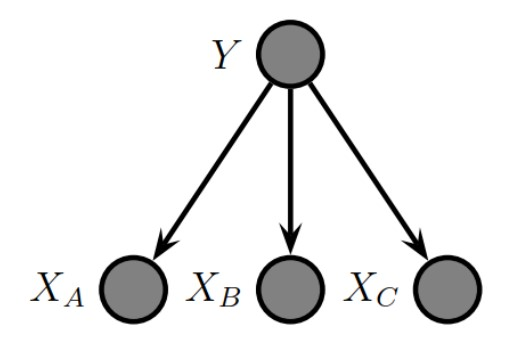
\includegraphics[width=0.5\textwidth]{a2_p12}
                \caption{The NBC graphical model}
            \end{figure}
            \begin{enumerate}[label=(\alph*)]
                \item Write down the joint probability of the random variables in the graph and factorize it according to the graph structure.
                \item For all pairs of features ($X_i$ and $X_j$, $i \neq j$),
                is $X_i \perp X_j | Y$? Explain what this means with respect to the problem of classification and the implications for the features.
                Is this true of our real data in practice?
                Can you think of a situation when this assumption will be explicitly violated, and may impact our classification accuracy? (answer in two sentences)
                \item We have a training set
                      $$
                      D_{training} = \{ (Y, X_A, X_B, X_C)_1, \dots, (Y, X_A, X_B, X_C)_n \}
                      $$
                    (with observed features and class lables, in other words, $n$ emails classified as spam or not spam), and a test set
                      $$
                      D_{test} = \{ (X_A, X_B, X_C)_{n+1}, \dots, (X_A, X_B, X_C)_{n+m} \}
                      $$
                    (with oberved features, but unknown class labels).\\
                    With this classifier, we could predict the probability that a test email belongs to the spam class. Write down how to compute $P(Y_j=1 | (X_A, X_B, X_C)_j)$, where $j=(n+1), (n+2), \dots (n+m)$, given that we know the components of our factorized joint probability.
            \end{enumerate}
        \end{problem}

        \begin{solution}
           \begin{enumerate}[label=(\alph*)]
               \item $Pr(Y, X_A, X_B, X_C) = Pr(Y) Pr(X_A|Y) Pr(X_B|Y) Pr(X_C|Y)$;
               \item Yes, $X_i \perp X_j | Y$; It means even when the spam email classification is given, we could not find any correlation among all the features. One practical example violates this assumption is that emails with all garbled words ($X_A = X_C$) must be spam mail with common knowledge;
               \item The computation is given below:
                    \begin{align*}
                        & Pr(Y_j=1 | (X_A, X_B, X_C)_j) \\
                        &= \frac{Pr((X_A, X_B, X_C, Y_j=1)_j)}{Pr((X_A, X_B, X_C)_j)} \\
                        &= \frac
                            {Pr(Y_j=1) Pr((X_A)_j|Y_j=1) Pr((X_B)_j|Y_j=1) Pr((X_C)_j|Y_j=1)}
                            {Pr(X_A) Pr(X_B) Pr(X_C)} \\
                        &= \pi \times
                            \frac
                            {
                                \prod_{k=\{A,B,C\}} (2\pi \sigma_{k,1}^2)^{-1/2}exp(\frac{(x-\mu_{k,1})^2}{2 \sigma_{k,1}^2})
                            }
                            {
                                \prod_{k=\{A,B,C\}} (2\pi \sigma_{k}^2)^{-1/2}exp(\frac{(x-\mu_{k})^2}{2 \sigma_{k}^2})
                            }
                    \end{align*}
           \end{enumerate}
        \end{solution}

        %=================== Problem 1.3 ===================%
        \begin{problem}
            [Maximum likelihood estimates for NBC]\\
            Still use the graph in Figure 3 and the task of classifying emails. Let's focus on the training data,
            $$
                D_{training} = \{ (Y, X_A, X_B, X_C)_1, \dots, (Y, X_A, X_B, X_C)_n \}
            $$
            Suppose our features $X_{A,B,C}$ in each class of emails have Gaussian distributions, e.g. $X_A|Y = y \overset{\mathrm{iid}}{\sim} \Gaussian(\mu_{A,y}, \sigma_{A,y}^2)$.
            In other words, the Gaussian parameters for the features are class-specific, meaning that there is one mean for feature $A$ when the email is spam and another mean for feature $A$ when it is not spam.
            \begin{enumerate}[label=(\alph*)]
                \item $Y \overset{\mathrm{iid}}{\sim} Ber(\pi)$, $\pi \in {[0, 1]}$. How do we find the MLE of $\pi$ using the training set $D$?
                \item If $\sigma_{A,y}^2$ is fixed, derive the MLE of $\mu_{A,1}$ and $\mu_{A,0}$ (in other words, the class mean of feature A for spam and not spam) using training set D.
                \item If $\mu_{A,1}$ and $\mu_{A,0}$ are fixed, derive the MLE for $\sigma_{A,0}^2$ using traning set D.
            \end{enumerate}
        \end{problem}

        \begin{solution}
            \begin{enumerate}[label=(\alph*)]
                \item Firstly we give out log likelihood with parameter $\pi$: $l(\pi) = log \prod_{i=1}^{n} Pr(Y^{(i)} | \pi)$; And for Bernoulli model, we have $\pi_{MLE} = \frac{\sum_{i=1}^{n} I[Y^{(i)}=1]}{N}$, where $I[Y^{(i)}=1]$ is indicator function with value 1 when the equality holds, and value 0 otherwise.

                \item Firstly we split the training set into two subset with respect to value of Y: $\{(Y=0, X_A, X_B, X_C)_{1}, \dots, (Y=0, X_A, X_B, X_C)_{n'}\}$ and $\{(Y=1, X_A, X_B, X_C)_{n'+1}, \dots, (Y=1, X_A, X_B, X_C)_{n}\}$.
                The log likelihood for $\mu_{A,0}$ is given as follow:
                \begin{align*}
                    l(\mu_{A,0}) &= \sum_{i=1}^{n'} log Pr(X_A^{(i)} | Y^{(i)=0}; \mu_{A,0}, \sigma^2_{A,0})
                    \\
                    &= -\frac{n'}{2} log(2\pi) - \frac{n'}{2} log(\sigma^2_{A,0}) - \frac{1}{2 \sigma^2} \sum_{i=1}^{n'} (X_A^{(i)} - \mu_{A,0})^2
                \end{align*}
                Then for Gaussian model, we have $\hat{\mu_{A,0}} = \frac{1}{n'} \sum_{i=1}^{n'} X_A^{(i)}$;\\
                And similarly for $\mu_{A,1}$ we have $\hat{\mu_{A,1}} = \frac{1}{n - n'} \sum_{i=n+1}^{n'} X_A^{(i)}$.

                \item With the definition introduced in previous problem (b), we could easily obtain MLE of $\sigma^2_{A,0}$ for the Gaussian model as: $\hat{\sigma^2_{A,0}} = \frac{1}{n'} \sum_{i=1}^{n'} (X_A^{(i)} - \hat{\mu_{A,0}})^2$
                
            \end{enumerate}
        \end{solution}
    \end{section}
    
    \begin{section}{Problem 2}
        \setcounter{pcounter}{0}
        We have studied in class how to construct generalized linear models (GLIM):
        $$
            \xi = \theta^T x, \mu=f(\xi), \eta=\psi(\mu)
        $$
        %=================== Problem 2.1 ===================%
        \begin{problem}
            [Poisson Regression]\\
            Under the framework, we want to model the data $\{(x_i, y_i)\}$ using Poisson as the conditional distribtuion of response variables $p(y|x, \lambda) = \frac{\lambda^y e^{-\lambda}}{y!}$.
            \begin{enumerate}[label=(\alph*)]
                \item Find the canonical response function $f(\cdot)$;
                \item Derive the batch gradient descent update rule;
                \item Derive the batch Newton descent update rule;
                \item Derive the stochastic gradient descent update rule.
            \end{enumerate}
        \end{problem}

        \begin{solution}
            \begin{enumerate}[label=(\alph*)]
                \item The Poission distribution could be written in canonical exponential family form as:
                $$
                    p(y|\eta) = \frac{1}{y!} exp (y \cdot \eta - exp(\eta))
                $$
                where $\eta = log{\lambda} = \theta^T x, \mu = exp(\eta)$; and we have $\mu = exp(\xi)$, where the canonical response function is $f(\cdot) = exp(\cdot)$;

                \item 
                As the conditional log likelihood is given by:
                \begin{align*}
                    J(\theta) &= log(\prod_{i=1}^{n} p(y_i | \eta_i)) \\
                    &= \sum_{i=1}^{n} log \frac{1}{y!} + \sum_{i=1}^{n}(\theta x_i y_i - exp(\eta_i))
                \end{align*}
                Then we have:
                \begin{align*}
                    \nabla_{\theta} J(\theta) &= \frac{\partial J(\theta)}{\partial \theta} \\
                    &= \sum_{i=1}^{n} (x_i y_i - \frac{\partial A(\eta_i)}{\partial \eta_i} \frac{\partial \eta_i}{\partial \theta}) \\
                    &= \sum_{i=1}^{n} x_i (y_i - u_i) \\
                    &= \sum_{i=1}^{n} x_i (y_i - exp(\theta^T x_i))
                \end{align*}
                The batch gradient descent algorithms follows:\\
                \begin{algorithm}[H]
                    \DontPrintSemicolon
                    \SetKwFunction{FMain}{GD}
                    \SetKwProg{Fn}{Function}{:}{}
                    \Fn{\FMain{$\mathcal{D}$, $\theta^{(0)}$}}{
                        $\theta \gets \theta^{(0)}$\;
                        \While{not converged}{
                            $\theta \gets \theta + \lambda \nabla_{\theta} J(\theta)$
                        }
                        \KwRet $\theta$\;
                    }
                \end{algorithm}
                
                \item The secoder differential could be obtained by:
                \begin{align*}
                    \nabla^2 J(\theta) &= \frac{\partial^2 J(\theta)}{\partial \theta^2} \\
                    &= - \sum_{i=1}^{n} x_i \frac{\partial \mu_i}{\partial \eta_i} x_i^T \\
                    &= - \sum_{i=1}^{n} x_i x_i^T exp(\theta^T x_i)
                \end{align*}
                The batch Newton descent algorithm follows:\\
                \begin{algorithm}[H]
                    \DontPrintSemicolon
                    \SetKwFunction{FMain}{NGD}
                    \SetKwProg{Fn}{Function}{:}{}
                    \Fn{\FMain{$\mathcal{D}$, $\theta^{(0)}$}}{
                        $\theta \gets \theta^{(0)}$\;
                        \While{not converged}{
                            $\theta \gets \theta + \lambda {{\nabla^2_{\theta} J(\theta)}^{-1}}{\nabla_{\theta} J(\theta)}$
                        }
                        \KwRet $\theta$\;
                    }
                \end{algorithm}
                
                \item The stochastic gradient descent algorithm follows:\\
                \begin{algorithm}[H]
                    \DontPrintSemicolon
                    \SetKwFunction{FMain}{SGD}
                    \SetKwProg{Fn}{Function}{:}{}
                    \Fn{\FMain{$\mathcal{D}$, $\theta^{(0)}$}}{
                        $\theta \gets \theta^{(0)}$\;
                        \While{not converged}{
                            \For{i $\in$ shuffle($\{1, 2, \dots, N\}$)}{
                                $\theta \gets \theta + \lambda \nabla_{\theta} J^{(i)}(\theta)$
                            }
                        }
                        \KwRet $\theta$\;
                    }
                \end{algorithm}
                where $\nabla_{\theta} J^{(i)}(\theta) = x_i (y_i - exp(\theta^T x_i))$.
            \end{enumerate}
        \end{solution}

        %=================== Problem 2.2 ===================%
        \begin{problem}
            [Multi-class Logistic Regression]\\
            As we discussed in class, we can also use category distribution GLIM to generalize logistic regression to multi-class classification.
            \begin{enumerate}[label=(\alph*)]
                \item Follow what we discussed in class, write down the MLE using the category distribution GLIM;
                \item Derive the batch gradient descent update rule.
            \end{enumerate}
        \end{problem}

        \begin{solution}
            \begin{enumerate}[label=(\alph*)]
                \item As category distribution GLIM could be written into exponential family form like:
                \begin{align*}
                    Pr(X=x) &= exp(\sum_{i=1}^{K} I[x=i] log p_i) \\
                    &= exp(\sum_{i=1}^{K-1} I[x=i] log{\frac{p_i}{p_K}} + log{p_K})
                \end{align*}
                where $\eta = [log{\frac{p_1}{p_K}}, \dots, log{\frac{p_{K-1}}{p_K}}]^T$ and $y = \{I[x=1], \dots, I[X=K-1]\}^T$;\\
                As $\mu = [p_1, \dots, p_{K-1}]^T$ and $\eta_i = log{\frac{p_i}{p_K}} = \theta_i^T x$, the differential of log likelihood function could be expressed as:
                \begin{align*}
                    \nabla_\theta J(\theta) &= \sum_{i=1}^{n} x_i(y_i - \mu_i) \\
                    &= \sum_{i=1}^{n} x_i \sum_{k=1}^{K-1} (I[x^{(i)}=k] - p^{(i)}_k)
                \end{align*}
                By setting $\nabla_\theta J(\theta) = 0$ we could obtain MLE for categorical distribtuion GLIM as:
                \begin{align*}
                    \hat{\mu_{MLE}} &= \frac{1}{n} \sum_{i=1}^{n} T(x_i) \\
                    &= [\sum_{i=1}^{n} I(x^{(i)}_1=1), \dots, \sum_{i=1}^{n} I(x^{(i)}_{K-1}=1)]^T
                \end{align*}
                
                \item The batch gradient descent algorithm follows:\\
                \begin{algorithm}[H]
                    \DontPrintSemicolon
                    \SetKwFunction{FMain}{GD}
                    \SetKwProg{Fn}{Function}{:}{}
                    \Fn{\FMain{$\mathcal{D}$, $\theta^{(0)}$}}{
                        $\theta \gets \theta^{(0)}$\;
                        \While{not converged}{
                            $\theta \gets \theta + \lambda \nabla_{\theta} J(\theta)$
                        }
                        \KwRet $\theta$\;
                    }
                \end{algorithm}
            \end{enumerate}
        \end{solution}
    \end{section}

    \begin{section}{Problem 3}
        \setcounter{pcounter}{0}
        %=================== Problem 3.1 ===================%
        \begin{problem}
            [Linear Regression]\\
            Some researchers who are desperately in need of a machine learning expert bring you a dataset with information on $n = 1100$ people.
            Their study has two explanatory predictors: $X_1=a$ binary indicator of gender (female=1 and male=0), and $X_2=$ some weight.
            They want to use this information to help predict blood pressure $Y$ which they believe is linearly related to $X_1$ and $X_2$.
            
            Suppose that $\sigma^2 = 1$ and for part (c) $\tau^2=1$. Use the first 1000 records for your training set, and the last 100 records for your test set.
            For this answer, \textbf{include your code (R, Matlab, python, etc.) in your solution}, but please do not use built in functions for linear regression. The dataset is HW2\_linear\_regression.txt.
            \begin{enumerate}[label=(\alph*)]
                \item Write a program to estimate $\beta$ using the \textbf{normal equation}. Estimate $\beta$ from the training set.
                \item Write a program to estimate $\beta$ usign \textbf{stochastic gradient descent}. Estimate $\beta$ from the tranining set.
                \item Write a program to estimate $\beta$ using the \textbf{ridge regression normal eqaution}. Estimate $\beta$ from the training set.
            \end{enumerate}
            For all of the above estimation procedures:
            \begin{enumerate}[resume, label=(\alph*)]
                \item Calculate $RSS(\hat{\beta}) = \frac{1}{n} \sum_{i=1}^{n} (y_i - \hat{\beta} x_i)^2$ in the training dataset;
                \item Calculate $RSS(\hat{\beta})$ in the test dataset;
                \item For each of the estimated values of $\hat{\beta}$, what is $E[Y|X=[1,135]^T, \hat{\beta}]$ ?
            \end{enumerate}
        \end{problem}

        \begin{solution}
            \begin{enumerate}[label=(\alph*)]
                \item The program using \textbf{normal euqation} is attached as \textbf{a2\_3\_normal.m};\\
                The estimated result is: $\hat{\beta} = [69.9422; 15.1191; 0.3210]$
                
                \item The program using \textbf{SGD} is attached as \textbf{a2\_3\_sgd.m};\\
                The estimated result is: $\hat{\beta} = [69.2205; 14.9835; 0.3272]$ (with fixed step size as $10^{-6}$ and stop criteria with $10^{-5}$);
                
                \item The program using \textbf{ridge regression normal equation} is attached as \textbf{a2\_3\_ridge.m};\\
                The estimated result is: $\hat{\beta} = [65.9129; 14.3522; 0.3479]$ with $\lambda=1$;
                
                \item $RSS(\hat{\beta})$ for training set: $98.7293$ for (a); $98.7866$ for (b); $99.0059$ for (c);
                \item $RSS(\hat{\beta})$ for test set: $115.7324$ for (a); $115.5875$ for (b); $115.2347$ for (c);
                \item $E[Y|X=[1,135], \hat{\beta}]$: $128.4001$ for (a); $128.3729$ for (b); $127.2297$ for (c);
            \end{enumerate}
        \end{solution}

        %=================== Problem 3.2 ===================%
        \begin{problem}
            [Logistic Regression]\\
            The researchers this time are interested in doing prediction for a binary outcome $Z$ (an indicator of adverse reaction to a drug they are testing), which they again beleive is linearly related to $X_1$ and $X_2$.\\
            Again, use the first 1000 records for your training set, and the last 100 records for your test set. The dataset is in HW2\_logistic\_regression.txt.
            \begin{enumerate}[label=(\alph*)]
                \item Write a program to estimate $\beta$ using the alogrithm introduced in class. Estimate $\beta$ using the training data;
                \item Calculate $RSS(\hat{\beta})$ in the training dataset;
                \item Calculate $RSS(\hat{\beta})$ in the test dataset;
                \item What is $E[Z|X=[1,135]^T, \hat{\beta}]$?
            \end{enumerate}
        \end{problem}

        \begin{solution}
            \begin{enumerate}[label=(\alph*)]
                \item The program with \textbf{Newton-Raphon Descent} algorithm is attached as \textbf{a2\_3\_logistic.m};
                \item $RSS(\hat{\beta})$ for training set: $3.9255$;
                \item $RSS(\hat{\beta})$ for test set: $3.8566$;
                \item $E[Y|X=[1,135], \hat{\beta}] = -2.3461$; 
            \end{enumerate}
        \end{solution}
    \end{section}

\end{document}